\chapter{Antecedentes}
\label{chap:antecedentes}

En este capítulo se discutiran algunos de los conceptos que se han empleado para la elaboración de este proyecto. En concreto, se hablará sobre las imágenes clínicas, estándar \acs{DICOM}, el entorno hospitalario y \acs{IHE}.

\section{Imagen médica}

\subsection{Origen e importancia de la imagen médica}

El cuerpo humano es un sistema increíblemente complejo. La adquisición de datos sobre sus propiedades estáticas y dinámicas se traduce en enormes cantidades de información. Uno de los mayores retos para investigadores y clínicos es la cuestión sobre cómo adquirir, procesar y visualizar la información sobre el cuerpo de forma que ésta pueda ser asimilada, interpretada y utilizada para ofrecer más métodos de diagnóstico y procedimientos terapéuticos útiles. En muchos casos, la presentación de la información como imagen es la aproximación más eficiente para abordar este reto, pues es un medio bastante confiable para la intervención en procesos de enfermedades y lesiones\cite{3}.

El descubrimiento de la imagen médica como prueba diagnóstica no sucedió hasta 1895 de la mano del físico Wilhelm Röntgen, que experimentaba con rayos catódicos obtenidos al aplicar descargas eléctricas en tubos de descarga gaseosa de alto voltaje (tubos de Crookes). Röntgen observó que estos rayos al atravesar una placa de platino-cianuro de bario emitían una luz fluorescente capaz de atravesar algunos objetos, dejando su sombra grabada en placas fotográficas. Denominó a esta luz fluorescente o radiación, rayos X y por este hallazgo recibió en 1901 el Premio Nobel de física. El uso de los rayos X proporcionaba estudios anatómicos "in vivo" pero como consecuencia se observó que en algunos casos producía efectos nocivos como radiodermitis y quemaduras, por lo que se pudo deducir que \textbf{las radiaciones no eran inocuas al cuerpo humano} \cite{4}.

Con el tiempo, las técnicas empleadas para la adquisición de imágenes médicas han ido evolucionando (con nuevos descubrimientos como los rayos Y (gamma), la radiación electromagnética, etc.) y disminuyendo su impacto sobre la salud del paciente. En los años 60 se comenzaron a usar pantallas intensificadoras permitiendo minimizar la dosis para obtener una imagen de calidad. A partir de los años 70 con la aparición de la tomografía axial computarizada (TAC) se inició la tendencia del uso de la imagen digital médica y comenzó a disminuir la radiografía convencional, evitando así problemas relacionados con la gestión y el tratamiento de las imágenes, como por ejemplo la repetición de pruebas y otros.

\subsection{Definición y características fundamentales}
Una imagen médica es la representación de la distribución espacial de una o más propiedades físicas o químicas dentro del cuerpo humano. Es decir, es una representación del interior del cuerpo obtenida de forma no invasiva, que ofrece información sobre su estructura y funcionamiento y mediante la que es posible detectar anomalías en el organismo. Las imágenes son capturadas mediante equipos o modalidades de adquisición de imagen \footnote{En el subapartado 3.1.3 se explica detalladamente este concepto}. Cada una de estas modalidades presenta diferentes técnicas físicas para distintos propósitos, en función de la información necesaria para la elaboración del diagnóstico al \cite{5}.

Para evaluar la \textbf{calidad de las imágenes médicas} se presta especial atención a dos características fundamentales, la resolución espacial y el contraste (o resolución de contraste). \footnote{Si bien existen otros parámetros implicados como la relación-ruido y los artefactos no se entra en detalle, puesto que no pueden valorarse directamente sobre la imagen y precisan que ésta sea manipulada posteriormente. Además, los parámetros aquí definidos presentan una relación más directa con el nivel de dosis inducido al paciente, objeto real de este trabajo \cite{6}}Otra característica importante es la resolución temporal, ya que es determinante en algunas modalidades para obtener una óptima calidad de imagen. Gracias a estos parámetros es posible evaluar la fidelidad y la riqueza de la información contenida en la representación de los objetos de estudio \cite{6} \cite{7}.

\begin{definitionlist}
\item La \textbf{resolución espacial} es una medida de la capacidad de una modalidad de imagen para producir imágenes de objetos en función de sus tamaños. El límite de resolución espacial clásico \footnote{La capacidad del ojo humano de discernir entre dos objetos} se encuentra en la mínima distancia a la que dos objetos pueden situarse de forma que en la imagen puedan ser distinguidos por separado.
\item La \textbf{resolución de contraste} permite distinguir en la imagen objetos o áreas que corresponden a zonas del objeto original con propiedades similares. Dado que la mayoría de las imágenes médicas son en blanco y negro, el contraste se suele manifestar en forma de niveles de grises. El contraste surge por diferentes propiedades de los tejidos, en función de la técnica de imagen empleada.
\item La \textbf{resolución temporal} es la capacidad para adquirir una imagen óptima en el
menor tiempo posible. En equipos con imágenes dinámicas o funcionales \footnote{Este tipo de imagen se define en el siguiente subapartado} , la resolución temporal es un parámetro aún más importante, pues trata de valorar el movimiento de un órgano, vaso o área lesionada.
\end{definitionlist}

El \textbf{caso ideal} para obtener imágenes de alta calidad es disponer de una \textbf{alta resolución espacial, de contraste y temporal} además de presentar las mínimas interferencias en la imagen (ruido, señales, artefactos). Sin embargo, esto implicaría \textbf{aumentar la dosis de radiación} e incumplir con uno de los principios de la protección radiológica: lograr un diagnóstico eficiente con la menor dosis posible. \footnote{Criterio ALARA: As Low As Reasonably Achievable} (Figura \ref{fig:parametros}).

\begin{figure}[!h]
\begin{center}
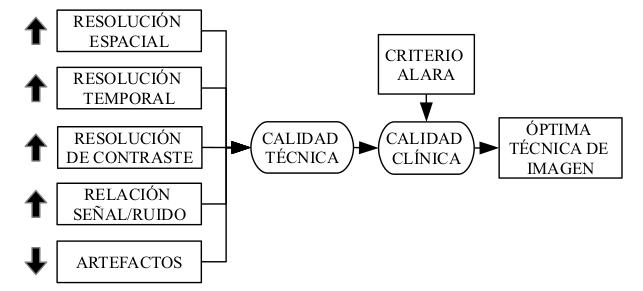
\includegraphics[width=0.75\textwidth]{images/parametros_image.jpg}
\caption{Relación entre parámetros para evaluar la calidad de la imagen médica}
\label{fig:parametros}
\end{center}
\end{figure}

\subsection{Modalidades de adquisición}
Las modalidades de adquisición hacen referencia a los equipos que toman las imágenes médicas de un paciente. Cada equipo utiliza sus técnicas y cálculos físicos para obtener una o varias imágenes del paciente que se somete a la prueba diagnóstica. La modalidad toma su nombre de la técnica empleada \cite{4}.

Como puede extrapolarse de su definición, el elemento básico que define una modalidad de adquisición determinada es es la \textbf{fuente de energía empleada}. La siguiente tabla (Tabla \ref{tab:modalidadesFundamentales}) recoge la clasificación de las modalidades fundamentales según la naturaleza de la energía:
\begin{table}[hp]
\centering{
\small



\begin{tabular}{p{.2\textwidth}p{.2\textwidth}}
  \tabheadformat
  \tabhead{Modalidad}   &
  \tabhead{Energía}      \\
\hline
Radiología 	     & Rayos X 	      \\
\hline
Medicina nuclear     & Rayos Y (gamma)    \\
\hline
Ecografía	     & Ultrasonidos	      \\
\hline
Resonancia magnética & Ondas de radio \\
\hline
\end{tabular}


% Local variables:
%   coding: utf-8
%   ispell-local-dictionary: "castellano8"
%   TeX-master: "main.tex"
% End:
}
\caption{Modalidades fundamentales según la fuente de energía}
\label{modalidadesFundamentales}
\end{table}

Por último, una clasificación muy interesante es \textbf{según la capacidad de separar objetos a diferentes profundidades:}
\begin{itemize}
\item Las \textbf{imágenes proyectivas}, son imágenes bidimensionales que constituyen la superposición de todas las estructuras del objeto representado.
\item Las \textbf{imágenes tomográficas}, representan múltiples planos o cortes de un mismo objeto, lo que facilita principalmente su interpretación al presentar menor superposición entre las estructuras que constituyen el objeto.
\end{itemize}
La tabla (Tabla \ref{tab:resumenModalidad}) resume la clasificación de las modalidades de imagen médica según las características presentadas anteriormente.

\begin{table}[hp]
\centering{
\small
\begin{tabular}{|c|c|c|c|c|c|}
\hline
\textbf{Modalidad}                             & \textbf{Técnica de imagen} & \textbf{Energía}             & \textbf{Radiación}                     & \textbf{Contraste}           & \textbf{Profundidad}         \\ \hline
\multirow{3}{*}{Radiología o Radiodiagnóstico} & Convencional               & \multirow{3}{*}{Rayos X}     & \multirow{5}{*}{\textbf{Ionizante}}    & \multirow{3}{*}{Morfológica} & \multirow{2}{*}{Proyectiva}  \\ \cline{2-2}
                                               & Digital                    &                              &                                        &                              &                              \\ \cline{2-2} \cline{6-6} 
                                               & TAC                        &                              &                                        &                              & \multirow{3}{*}{Tomográfica} \\ \cline{1-3} \cline{5-5}
\multirow{2}{*}{Medicina Nuclear}              & SPECT                      & \multirow{2}{*}{Rayos Y}     &                                        & \multirow{2}{*}{Funcional}   &                              \\ \cline{2-2}
                                               & PET                        &                              &                                        &                              &                              \\ \hline
Ecografía                                      & Ecografía                  & Ultrasonido                  & \multirow{4}{*}{\textbf{No ionizante}} & \multirow{2}{*}{Morfológica} & \multirow{3}{*}{Tomográfica} \\ \cline{1-3}
\multirow{2}{*}{Resonancia magnética}          & MRI                        & \multirow{2}{*}{Ondas radio} &                                        &                              &                              \\ \cline{2-2} \cline{5-5}
                                               & FMRI                       &                              &                                        & Funcional                    &                              \\ \cline{1-3} \cline{5-6} 
Endoscopia                                     & Endoscopia                 & Luz                          &                                        & Morfológica                  & Proyectiva                   \\ \hline
\end{tabular}
% Local variables:
%   coding: utf-8
%   ispell-local-dictionary: "castellano8"
%   TeX-master: "main.tex"
% End:
}
\caption{Resumen de la clasificación de las modalidades de adquisición. Destacado el tipo de radiación que inducen a un paciente, ionizante, no ionizante}
\label{resumenModalidad}
\end{table}

\subsubsection{Técnicas de adquisición de imágenes}
Desde la utilización del primer equipo de rayos X de Röntgen hasta la actualidad, se han desarrollado una gran variedad de equipos tanto en diseño como en su aplicación específica. Estos equipos se organizan en varios tipos de técnicas de obtención de imagen médica \cite{7} \cite{8}:
\begin{itemize}
\item \textbf{\underline{Radiología convencional:}} Consiste en proyecciones simples correspondientes a estructuras óseas y partes blandas del cuerpo (tórax, abdomen, columna, extremidades, etc). El receptor de imagen es una placa fotográfica. 

También son habituales en este tipo las \textbf{mamografías} (muy importantes para el diagnóstico y la prevención del cáncer de mama) y las \textbf{radiografías dentales} (las más comunes son las intraorales, las ortopantomografías y los TC dentales). 

Existen \textbf{equipos portátiles de radiología convencional} para llegar a aquellos pacientes hospitalizados que no pueden ser desplazados hasta los servicios de radiología.

\item \textbf{\underline{Fluoroscopía:}} El receptor de imagen es una pantalla fluorescente que se ilumina al proyectar sobre ella el haz de rayos X, por lo que las diferencias de intensidad de luz permiten distinguir las estructuras anatómicas. Con esta técnica se obtienen imágenes dinámicas en tiempo real que pueden visualizarse en un monitor de TV. La emisión de radiación puede prolongarse durante un tiempo con el fin de capturarimágenes fijas de la proyección seguida en el monitor de TV para el diagnóstico.

La Fluoroscopía es utilizada en los equipos denominados \textbf{telemandos} para obtener estudios más complejos del aparato digestivo y urinario. También se puede utilizar esta técnica en \textbf{arcos radioquirúrgicos} y en \textbf{angiógrafos vasculares y cardíacos} para guiar un catéter o un endoscopio introducido generalmente por vía vascular.

\item \textbf{\underline{Radiología digital:}} En esencia es igual a la radiología convencional salvo que el receptor de imagen utilizado es un detector electrónico de gran resolución a partir del cual se obtiene la imagen médica mediante medios informáticos. El origen de la radiografía digital ocurrió al mismo tiempo que el descubrimiento de la tomografía computarizada en los años 70, pues esta técnica necesitaba del ordenador para obtener las imágenes.

La radiología digital se utiliza en técnicas como el \textbf{TAC}, la \textbf{Angiografía digital} y la \textbf{Radiografía convencional} (incluyendo por supuesto la Mamografía y las radiografías dentales). 

Para el caso de la Radiología convencional, se han desarrollado dos nuevas tecnologías para obtener imágenes digitales de forma directa \cite{9}: 

\item \textbf{\underline{Radiografía computarizada (CR - Computed Radiography):}} Genera la
imagen a partir de unas placas especiales de fósforo, para después ser tratada en estaciones especiales donde se construye la imagen digital.
 
\textbf{\underline{Radiografía digital (DR - Digital Radiography):}}\footnote{El estándar DICOM hace referencia a esta técnica con el acrónimo DX (Digital X-Ray)} Utiliza unos receptores digitales basados en semiconductores que transforman directamente la energía
de rayos X en señales digitales.

La siguiente tabla (Tabla \ref{tab:modalidadImagen}) muestra algunos de los acrónimos para las técnicas de adquisición de imagen obtenidas mediante sistemas digitales \footnote{Acrónimos y nombres utilizados en concreto por el estándar de imagen médica digital DICOM}:

\begin{table}[hp]
\centering{
\small



\begin{tabular}{p{.2\textwidth}p{.2\textwidth}}
\hline
CR &Radiografía computarizada X\\
\hline
CT&Tomografía computarizada\\
\hline
DF&Fluoroscopía digital\\
\hline
MG&Mamografía\\
\hline
MG&Angiografía de susbtracción digital \\
\hline
\end{tabular}


% Local variables:
%   coding: utf-8
%   ispell-local-dictionary: "castellano8"
%   TeX-master: "main.tex"
% End:
}
\caption{Modalidades de imágenes médicas}
\label{modalidadImagen}
\end{table}

\item \textbf{\underline{Tomografía computarizada (TC o TAC):}} \footnote{TC(Tomografía computarizada) y TAC(Tomografía axial computarizada) son dos formas de nombrar la misma técnica. Actualmente se utiliza erróneamente la expresión TAC, porque la mayoría de estos equipos no sólo permite obtener cortes axiales del objeto de estudio sino también otros tipos de planos.} Permite obtener imágenes del objeto de estudio en diferentes planos (axial, sagital, coronal, etc.) lo que posibilita una visualización nítida de diversas estructuras anatómicas como: huesos, órganos, nervios, etc. que no pueden visualizarse con una imagen proyectiva típica de la radiografía convencional. Se utiliza un haz de rayos X muy estrecho que gira alrededor del cuerpo del paciente a medida que éste pasa por una abertura circular del equipo, estando tumbado en una mesa móvil.

	Las imágenes se construyen mediante cálculos matemáticos a partir de la información suministrada por una o varias filas de detectores distribuidos sobre un arco, que reciben la radiación dispersada por el organismo.

\item \textbf{\underline{Radiología intervencionista:}} Rama de la Radiología que utiliza procedimientos mínimamente invasivos en estudios del sistema circulatorio, tanto coronario, como neurológico, como periférico, evitando en muchos casos intervenciones quirúrgicas más invasivas.

	La imagen se obtiene mediante la inyección de un contraste, es decir, un buen absorbente de la radiación que produce una sombra visible. Esta sustancia es inyectada en la zona a explorar utilizando agujas o guiando un catéter con Fluoroscopía.

	La Radiología intervencionista se utiliza tanto para diagnóstico como para tratamientos terapéuticos. Esta técnica es utilizada por arcos radioquirúrgicos y los angiógrafos vasculares y cardíacos.
\end{itemize}

La imagen (Figura \ref{fig:tecnicasModalidad}) recoge un resumen de este subapartado, mostrando la evolución de la radiología convencional a la digital y en qué técnicas se encuentran los diferentes equipos o modalidades de adquisición de radiodiagnóstico.

\begin{figure}[!h]
\begin{center}
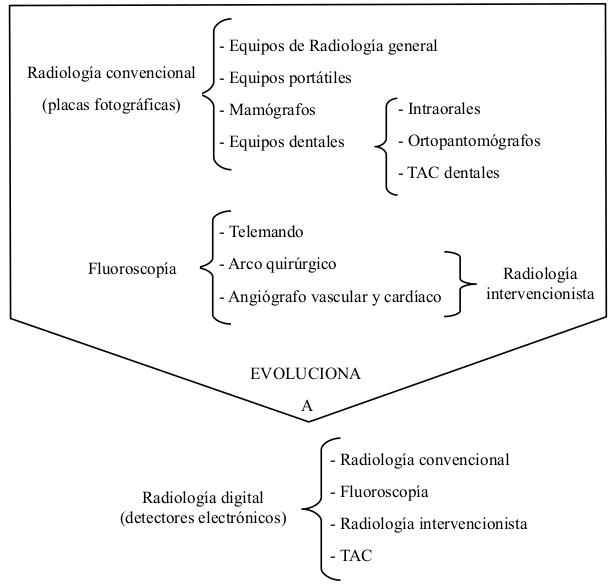
\includegraphics[width=0.75\textwidth]{images/tecnicas_modalidad.jpg}
\caption{Técnicas y modalidades de adquisición de imagen en Radiodiagnóstico}
\label{fig:tecnicasModalidad}
\end{center}
\end{figure}

\section{El estándar \acs{DICOM}}
\subsection{Orígenes del estándar}
Desde la aparición del TAC en los años 70 junto con otras modalidades de adquisición, el uso de las tecnologías en los entornos hospitalarios y clínicos ha ido en aumento. La interoperabilidad entre equipos de diferentes fabricantes se convirtió en un tema crítico, ya que cada fabricante presentaba sus formatos de imagen y servicios propios, dificultando enormemente la comunicación y el intercambio de datos. Siendo conscientes de esta situación, en 1983, el comité conjunto formado por ACR y NEMA comenzó a desarrollar el estándar \acs{DICOM}.

La primera versión del estándar, denominada ACR-NEMA 1.0 fue publicada en 1985. Pocos años después, en 1988, se publicó una versión más estable, ACR-NEMA 2.0. Sin embargo, debido a la rápida expansión de la red y la aparición de nuevas modalidades de adquisición a finales de los años 80, la versión ACR-NEMA 2.0 se quedó bastante limitada.

En 1993 se publicó la versión definitiva del estándar que cambió su nombre a ACR-NEMA \acs{DICOM} o como se le conoce actualmente \acs{DICOM} 3.0 o \acs{DICOM}. Desde entonces, se han ido publicando nuevas revisiones de la versión 3 casi anualmente, la más reciente de 2016 \footnote{Partes del estándar en su última revisión de 2016} \cite{1}.

\acs{DICOM} nunca ha sido reemplazado por una nueva versión. Las sucesivas actualizaciones del estándar son extensiones, no versiones, que se van ajustando a las prácticas clínicas del momento. Sin embargo, la especificación básica del estándar permanece inalterada. 

\subsection{Definición del estándar}
Este estándar presenta la definición de un \textbf{formato común de archivo de imagen} con dos partes bien diferenciadas: una \textbf{cabecera de datos} \footnote{En realidad, el término cabecera en el formato de archivo \acs{DICOM} no hace referencia a dicha información, sino a otros parámetros que indican el contexto en el que fue grabada la imagen, por ejemplo, que codificación se usó, que software grabó la información, etc. El término cabecera se utiliza por comodidad para referirse a todos los datos codificados en la imagen \acs{DICOM}, sean clínicos o de otro tipo. En el subapartado 3.2.4 se describe con detalle cómo se estructura el formato de archivo \acs{DICOM}. Hasta entonces se hará referencia a la cabecera como tal y como se describe aquí en la introducción.} que contiene información codificada relativa al paciente, a la modalidad de adquisición y a la imagen generada como resultado de la exploración; y la \textbf{imagen} en sí.

Además, proporciona todo lo necesario para la \textbf{representación precisa del diagnóstico} y el \textbf{tratamiento de datos} de imágenes médicas \cite{10}, pues:
\begin{itemize}
\item Da soporte a numerosos \textbf{parámetros de adquisición} de imagen (como la posición 3D del paciente, tamaños físicos de objetos en la imagen, parámetros de exposición de la imagen, etc.) y datos de diferentes tipos (fechas, tiempos, números reales, etc.).
\item Presenta un \textbf{diccionario de datos} que contiene la codificación de más de 2000 atributos sobre información médica.
\item Ofrece una \textbf{excelente calidad de imagen} aprovechando las últimas y más avanzadas técnicas de representación de imagen digital.
\end{itemize}

También presenta un \textbf{protocolo de comunicación específico}, basado en TCP/IP, que define un servicio de intercambio de mensajes entre equipos (que pueden o no transportar datos, según cual sea su cometido), y varias clases de servicios para la comunicación de información digital médica.

Algunas de las clases de servicios disponibles en \acs{DICOM} son \cite{1}:
\begin{itemize}
\item \textbf{\underline{Storage Service Class:}} Permite la transmisión de imágenes entre dos equipos.
\item \textbf{\underline{Query/Retrieve Service Class:}} Permite la búsqueda de imágenes de un sistema de información de gestión y almacenamiento, como es el \acs{PACS}, por petición de una estación de trabajo.
\item \textbf{\underline{Basic Worklist Management Service Class:}} Permite el acceso a las listas de trabajo. Una lista de trabajo presenta información relacionada con una lista de tareas a realizar (pacientes citados) para la modalidad.
\item \textbf{\underline{Print Management Service Class:}} Permite la impresión de las imágenes y los datos relacionados reflejados en la propia imagen en soportes estándares definidos, como por ejemplo placas de rayos X.
\end{itemize}

\acs{DICOM} permite integrar una gran variedad de equipos (modalidades de adquisición, \acs{PACS}, estaciones de trabajo, impresoras, etc.), tanto dentro como fuera de un entorno hospitalario, en un sistema de almacenamiento y comunicación de imágenes \cite{10}
\cite{11}.

Para conocer qué características de \acs{DICOM} soporta un equipo y si es compatible con el resto de los sistemas de información que se encuentran en una red hospitalaria, éste dispone de un documento denominado \textbf{\acs{DICOM} Conformance Statement (DCS)}. En él se  define el grado de compatibilidad que presenta con el estándar. Cada equipo tiene su propio DCS donde se especifican los objetos de información reconocidos, las clases de servicio, los protocolos de comunicación, los medios físicos y las medidas de seguridad soportadas \cite{12}.

\subsection{La información clínica en \acs{DICOM}}
\subsubsection{Del modelo del mundo real al modelo de información \acs{DICOM}}
Cuando un paciente llega a un centro hospitalario para realizarse una prueba en un equipo de adquisición de imágenes, se genera gran cantidad de información referente a todo el procedimiento desde que comienza la prueba hasta que ésta finaliza. No sólo se obtiene información sobre parámetros referentes a la técnica empleada al paciente, como el kilovoltaje, el tiempo de exposición, etc., sino también información referente a las entidades que participan y sus interrelaciones.

Toda esta información queda recogida de forma organizada en las cabeceras \acs{DICOM} de las imágenes médicas. Para ello, el estándar adopta el modelo del mundo real y lo transforma dando lugar a un modelo de información propio en el cual todo gira alrededor del paciente.

Un posible escenario del mundo real sería el siguiente. El \textbf{paciente} llega al equipo donde se va a realizar una prueba, denominada \textbf{estudio}. Tras la realización de ese estudio, se obtienen una o varias series de imágenes médicas. Cada \textbf{serie} puede contener, a su vez, una o varias imágenes. Por tanto se puede ver cómo la \textbf{imagen} está relacionada con cada una de las entidades aquí descritas. Por ejemplo, un estudio es un TAC de abdomen. El estudio se compone de varias series, una primera serie resumen de una imagen y otra serie con 128 cortes de la región abdominal. O bien, un estudio de una rodilla que se compone de dos series, una que contiene una imagen de un lado de la rodilla (lateral derecho o izquierdo) y otra imagen de frente.

A partir del escenario anterior es fácil obtener un modelo de información que lo represente, tal cual se muestra en la siguiente figura (Fig.\ref{fig:mundoReal_modelo}). Esta jerarquía de clases formada por las entidades Paciente-Estudio-Serie-Imagen es el esqueleto básico para organizar la información contenida en las cabeceras DICOM de las imágenes \cite{10}. El estándar suma un nivel más de complejidad en el modelo de información anterior y aplica un análisis orientado a objetos para definir un diagrama de entidad-relación (ER) y así modelar las entidades del mundo real como objetos abstractos, además de conocer la forma en que estos objetos están relacionados \cite{13}.

\begin{figure}[!h]
\begin{center}
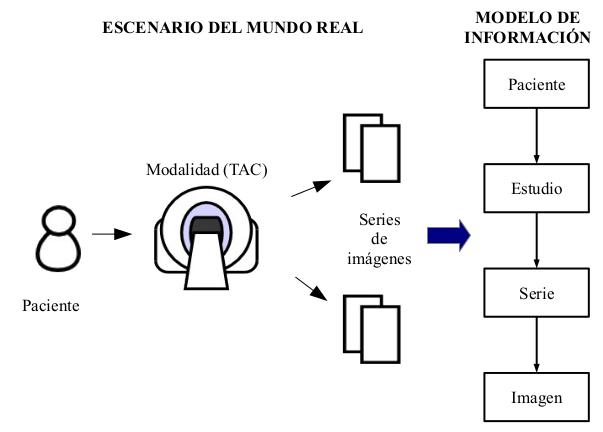
\includegraphics[width=0.75\textwidth]{images/mundoReal_modelo.jpg}
\caption{Del mundo real al modelo de información DICOM}
\label{fig:mundoReal_modelo}
\end{center}
\end{figure}

En la figura (Fig. \ref{fig:ER_DICOM}) se describe el modelo \acs{ER} adoptado por \acs{DICOM}, con algunas de las entidades de información (\acs{IE}) participantes en el flujo de trabajo de la imagen médica. En la especificación del estándar hay definidas alrededor de 20 IEs \cite{13}, sin embargo, esta lista se encuentra en continua actualización por los DICOM WGs \footnote{DICOM WG, (work group) son equipos de trabajo dedicados a mejorar diferentes partes del estándar. Cada grupo atiende a un dominio en concreto (modalidades, dominio clínico, funciones). Por ejemplo, el WG-06 se encarga de la base del estándar. Ver documento estratégico del estándar: \url{http://medical.nema.org/dicom/geninfo/Strategy.pdf}}.

Gracias a este modelo ER se pueden definir objetos de información y además identificar los atributos que los constituyen. Estos objetos se denominan \textbf{\acs{IOD} (Information Object Definition)}.

\begin{figure}[!h]
\begin{center}
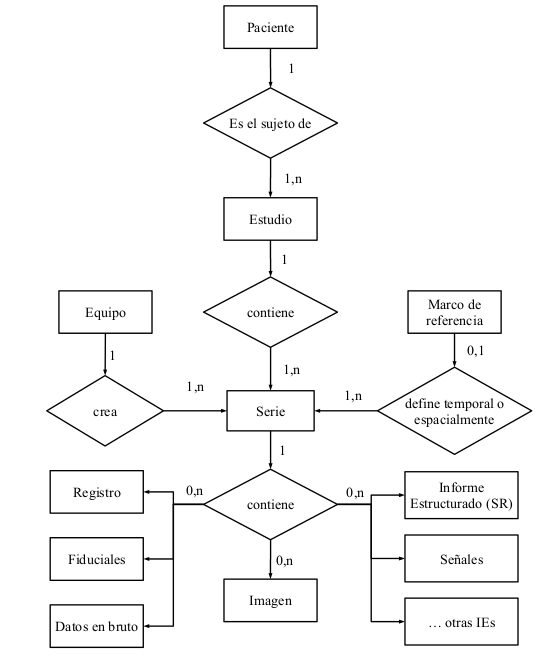
\includegraphics[width=0.85\textwidth]{images/ER_DICOM.png}
\caption{Modelo ER DCIOM - Representación de la iformación clínica}
\label{fig:ER_DICOM}
\end{center}
\end{figure}

\subsubsection{Definición de objeto de información (IOD)}
Una definición de un objeto de información (\acs{IOD}) es la representación abstracta de un objeto del mundo real que contiene la información necesaria para su descripción semántica, es decir, un conjunto de atributos que describen las características del objeto y las relaciones que presenta con otros objetos asociados.

Un \acs{IOD} puede verse como una plantilla de atributos o una clase de la cual se pueden crear instancias de ese objeto de información. Dicha plantilla agrupa de forma ordenada los atributos en \textbf{módulos de información}, y a su vez, varios módulos representan una \textbf{entidad de información (\acs{IE})}. La figura (Fig. \ref{fig:def_IOD}) muestra qué elementos incluye un \acs{IOD}.

\begin{figure}[!h]
\begin{center}
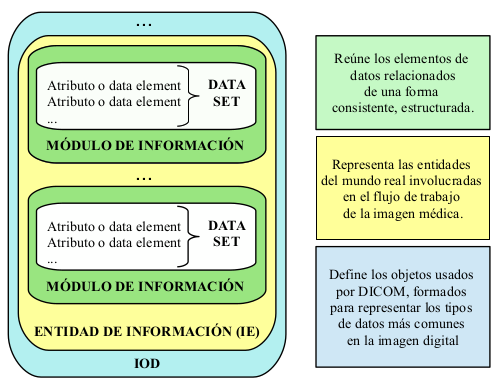
\includegraphics[width=0.65\textwidth]{images/def_bas_IOD.png}
\caption{Definición básica de un \acs{IOD}}
\label{fig:def_IOD}
\end{center}
\end{figure}

El estándar DICOM clasifica los IODs en normalizados y compuestos \cite{11} \cite{13}:

\begin{itemize}
\item \textbf{\underline{Normalizado:}} Representa una única entidad del mundo real, como por ejemplo Patient IOD que representa sólo a la entidad paciente.
\item \textbf{\underline{Compuesto:}} Representa a varias entidades de información, como por ejemplo CT Image IOD (una imagen de TAC) que, además de contener atributos de la entidad imagen, incluye otros atributos de otras entidades relacionadas como paciente, estudio, equipo, etc. Los IODs compuestos son más adecuados para la captura de interrelaciones, asociaciones, procesos y contextos.
\end{itemize}

Cada tipo de IOD tiene asociado un conjunto de acciones para operar sobre ellos, pero esto se verá con más detalle en el subapartado 3.2.3 sobre la comunicación en DICOM.

\subsubsection{Estructura de los datos en \acs{DICOM}}
Los atributos pertenecientes a un objeto del mundo real son codificados en \acs{DICOM} como \textbf{elementos de datos} (data elements), ver (Fig. \ref{fig:ER_DICOM}). Éstos son registrados en un \textbf{diccionario de datos} propio del estándar, donde se recoge la colección de todos los tipos de elementos de datos disponibles para representar la información \cite{14}. Su contenido específico y su semántica se encuentra especificado en las IODs. Un elemento de dato está registrado en el diccionario de datos siguiendo esta estructura (Tabla \ref{tab:camposIOD}):

\begin{table}[hp]
\centering{
\small
\begin{tabular}{|c|c|c|c|c|}
\hline
\begin{tabular}[c]{@{}c@{}}Tag\\ (gggg,eeee)\end{tabular} & Attribute Name & VR & VM & Value \\ \hline
\end{tabular}
% Local variables:
%   coding: utf-8
%   ispell-local-dictionary: "castellano8"
%   TeX-master: "main.tex"
% End:
}
\caption{Campos que denominan a un elemento de datos en el diccionario estándar}
\label{tab:camposIOD}
\end{table}

Cada elemento de dato se identifica de forma unívoca por una \textbf{etiqueta o tag}. El tag consiste en un par ordenado de números expresados en hexadecimal que representa el \textbf{número de grupo} seguido del \textbf{número del elemento}. Se presenta como (gggg, eeee) y según el número de grupo se puede diferenciar a que tipo de elemento de dato pertenece \cite{15}:
\begin{itemize}
\item \textbf{\underline{Comando:}} Corresponde con los grupos \textbf{(0000, eeee), (0002, eeee), (0004, eeee) y (0006, eeee)} y están reservados para los comandos utilizados en el intercambio de mensajes entre equipos. No están registrados en el diccionario de datos, sino que se describen en la parte 7 (PS3.7) del estándar, en el anexo E \cite{16}.
\item \textbf{\underline{Privado:}} \textbf{Su número de grupo es impar} y está reservado a los fabricantes de modalidades de adquisición para incluir sus datos propietarios en las cabeceras DICOM. Sin embargo, ningún elemento de dato privado puede pertenecer a los siguientes grupos: (0001, eeee), (0003, eeee), (0005, eeee), (0007, eeee), (FFFF,eeee).
\item \textbf{\underline{Estándar:}} Corresponde con los \textbf{grupos pares} restantes que se encuentran en la colección de elementos de datos registrada en el diccionario de datos. De cualquier forma, todos los grupos pares están reservados para uso estándar de cara a futuras
extensiones del estándar.
\end{itemize}

El \textbf{VR} es el valor de representación que toma el elemento de dato. Existen 27 tipos básicos definidos por el estándar DICOM, para representar los distintos formatos posibles \footnote{Listado completo de los tipos de valores de representación definidos por el estándar DICOM. (VéaseAnexo B).} , entre ellos se encuentran varios formatos de texto, número, fecha, hora, edad, binario, identificadores únicos, etc.

El \textbf{VM} es el valor de multiplicidad , es decir, define el número de valores de su tipo (VR) que puede contener este elemento. DICOM concatena los valores múltiples en un sólo valor multivaluado, si el VR es de tipo texto se usa como delimitador un backslash "\", si se trata de un VR binario no se usa delimitador, ya que la longitud de cada valor individual es conocida y fija.

\subsubsection{Codificación de los datos a objetos \acs{DICOM}}
Un \textbf{objeto \acs{DICOM}} constituye la \textbf{parte más esencial de la estructura del estándar}. Todos los datos \acs{DICOM} (comandos, informes, imágenes médicas, etc) se encuentran siempre encapsulados en un formato de objeto \acs{DICOM}. En este formato, los objetos pueden viajar entre varios dispositivos conectados a una red \acs{DICOM} y ser almacenados en archivos \acs{DICOM}. Es decir, un objeto DICOM no es más que una \textbf{colección de elementos} de datos, por tanto no existe una cabecera DICOM y una imagen DICOM separadas \footnote{Las imágenes médicas codificadas en objetos DICOM tienen asignados varios elementos de datos del diccionario estándar. Algunos de ellos son la altura de la imagen en (0028,0010) Rows, el ancho: (0028,0011) Columns y los datos de pixel de la imagen: Pixel Data (7FE0,0010), es decir la imagen en sí que se visualiza. La imagen suele ocupar el 95\% del tamaño del objeto DICOM.}, sino que ambas constituyen el objeto DICOM global \cite{10}.

Cada uno de los elementos de datos individuales que constituyen el conjunto de datos codificado en un objeto DICOM, conserva prácticamente la misma organización en campos que se especifica en su definición para el diccionario de datos estándar. En este caso (Tabla \ref{tab:camposDICOM}) se incluye la longitud en bytes del elemento de dato, pero se excluye el campo del nombre del atributo, pues las aplicaciones DICOM que interpretan estos objetos se refieren a los elementos de datos por su tag y no por su nombre descriptivo \cite{15}.

\begin{table}[hp]
\centering{
\small
\begin{tabular}{|c|c|c|c|}
\hline
\begin{tabular}[c]{@{}c@{}}Tag\\ (gggg,eeee)\end{tabular} & VR & Lenght & Value \\ \hline
\end{tabular}
% Local variables:
%   coding: utf-8
%   ispell-local-dictionary: "castellano8"
%   TeX-master: "main.tex"
% End:
}
\caption{Campos que denominan a un elemento de dato codificado dentro de un objeto DICOM}
\label{tab:camposDICOM}
\end{table}

Cuando los elementos de datos son codificados a objetos DICOM, el \textbf{orden de grabación es estricto}, empezando por el más pequeño en relación al par (grupo, elemento). Es decir, dentro de cada grupo los elementos están ordenados de manera \textbf{ascendente}, y los grupos están ordenados en orden de grupo ascendente.

La siguiente lista de elementos de datos (Fig. \ref{fig:fragDatos}) corresponde a un fragmento de la cabecera DICOM de una imagen, extraídos con la utilidad dcm2txt dentro del toolkit de dcm4che2. \footnote{En el capítulo 4 se describe en detalle en que consiste este toolkit dcm4che2.} En él se aprecia el orden de grabación de los elementos de datos. El formato de salida de la cabecera DICOM corresponde a los campos, por orden de aparición, tag, VR, longitud, valor, y nombre del atributo. Esta utilidad proporciona un formato de las cabeceras DICOM legible al usuario, respetando el orden de codificación.

\begin{figure}[!h]
\begin{center}
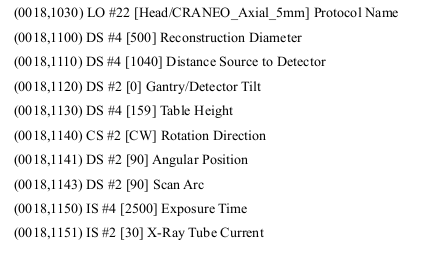
\includegraphics[width=0.65\textwidth]{images/fragDatos.png}
\caption{Fragmento de los datos contenidos en la cabecera \acs{DICOM} de una imagen. Imagen perteneciente al corte axial de un TAC de cabeza (HGUCR)}
\label{fig:fragDatos}
\end{center}
\end{figure}

DICOM define textbf{dos tipos de codificación: Implicit VR y Explicit VR}. El tipo Implicit es la codificación más simple, y es usada como la codificación por defecto en DICOM. A su vez, para cada codificación se determina el \textbf{orden de bytes: Little Endian} (por defecto en DICOM) y \textbf{Big Endian}. Por tanto el método de codificación por defecto en DICOM es Implicit VR Little Endian.

\subsubsection{Clasificación de los elementos de datos}
Los atributos codificados como elementos de datos pueden ser o no requeridos en un conjunto de datos dependiendo del tipo de elemento de dato al que correspondan. Estos tipos se utilizan para especificar si un elemento es \textbf{requerido, condicional u opcional}. En concreto, DICOM define los siguientes tipos de elementos de datos: 

\begin{itemize}
\item \textbf{\underline{Tipo 1:}} Son obligatorios. El campo “valor” debe tener un valor válido. La longituddel campo no puede ser 0.
\item \textbf{\underline{Tipo 1C:}} Son obligatorios si se cumplen las condiciones a las que estén sujetos. En ese caso, el campo “valor” debe tener un valor válido y la longitud del campo no puede ser 0.
\item \textbf{\underline{Tipo 2:}} Son obligatorios, pero el campo “valor” puede presentar un valor válido o ninguno y ser de longitud 0 si el valor es desconocido.
\item \textbf{\underline{Tipo 2C:}} Presenta los mismos requisitos que el tipo 2, pero si cumple las condiciones a las que está sujeto.
\item \textbf{\underline{Tipo 3:}} Son opcionales. El elemento de datos puedo o no estar incluido en el conjunto de datos y si lo esta puede ser de longitud 0.
\end{itemize}

En cada una de los IODs definidos en la parte 3 del estándar (PS3.3) \cite{13} también se especifica una clasificación similar, indicando el uso que se pueden hacer de los módulos de información que éstos incluyen. Así, los módulos pueden ser de uso obligatorio (M = mandatory), condicional (C = Conditional) o definido por el usuario (U = user-defined).

\subsubsection{Identificadores únicos (UID)}
Para identificar de forma unívoca cada una de las instancias particulares que constituyen un objeto DICOM, el estándar determina un elemento de dato clave para cada una de ellas, formateado con el valor de representación \textbf{(VR) UID.}

Con este identificador en DICOM se definen y registran imágenes individuales, series de imágenes, estudios, dispositivos, sintaxis en los protocolos de intercambio de imágenes, clases SOP (par servicio-objeto), y otros muchos elementos. 

Un UID DICOM es una cadena de texto codificado que presenta esta sintaxis \cite{15}:
\begin{listing}[
	float=ht,
	lenguage = marcas,
	caption = {},
	label = code:org_suffix]
	<org.root>.<suffix>.
\end{listing}

\begin{itemize}
\item La parte \textbf{<org.root>} identifica una organización (por ejemplo fabricante, organización de investigación, NEMA, etc.). El <org.root> \textbf{"1.2.840.10008"} está reservado para todos los UIDs de transacción DICOM y no se usaría por otros elementos definidos como privados (como la instancia de una imagen).

\item La parte \textbf{<suffix>} está formada por varios componentes numéricos y debe ser único dentro del ámbito del <org.root>.
\end{itemize}

En el anexo A de la parte 6 del estándar (PS3.6) \cite{14}, correspondiente al diccionario de datos de DICOM, se encuentran el registro de todos los valores UID del estándar.

Un ejemplo de un UID registrado en el estándar es el identificador para el almacenamiento de imágenes de TAC (CT Image Storage): 1.2.840.10008.5.1.4.1.1.2 

Los \textbf{UIDs} son utilizados a menudo \textbf{como nombres de archivo DICOM}. En concreto, se utiliza como nombre el elemento de dato Image SOP Instance UID con el tag (0008,0018) ya que es una manera fácil de identificar una imagen DICOM almacenada en un soporte físico. En este UID, la parte <suffix> puede contener datos de identificación del equipo o de la propia imagen. Un ejemplo de ello sería:

1.2.840.113704.7.1.1.2024.1339005147.2, donde 1.2.840.113704 corresponde a una organización específica, en este caso al fabricante Philips \footnote{Idealmente cada organización registra su propio identificador <org.root> para garantizar que ese identificador no está en uso para el resto. En el siguiente enlace se pueden consultar algunos identificadores registrados: \url{http://www.oid-info.com}}.

\section{La comunicación en DICOM}
\subsection{Introducción}
\subsubsection{El protocolo de comunicación DICOM}
DICOM utiliza el modelo TCP/IP para definir su propio lenguaje de red, que especifica cómo formatear e intercambiar objetos DICOM (imágenes médicas y su información asociada) entre equipos dentro de un entorno hospitalario o incluso fuera de él (por ejemplo la telemedicina). Como resultado, el modelo TCP/IP ve aumentada su funcionalidad al añadir una capa de aplicación DICOM con protocolos específicos \cite{10} \cite{17}.
La capa de aplicación DICOM se organiza en dos niveles (Fig. \ref{fig:integracionDICOM}):
\begin{itemize}
\item El nivel superior presenta los servicios de alto nivel, que consiste en las clases SOP (Service-Object Pair) y el protocolo DIMSE (DICOM Message Service Element).
\item El nivel inferior presenta los servicios de bajo nivel, que consisten en primitivas para la negociación de la asociación entre entidades de aplicación y el intercambio de estructuras para la gestión de dicha asociación (PDU, Protocol Data Unit). Esta capa es conocida como el protocolo DICOM Upper Layer (DICOM UL).
\end{itemize}

\begin{figure}[!h]
\begin{center}
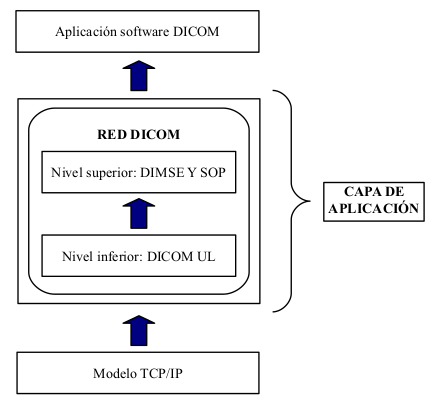
\includegraphics[width=0.65\textwidth]{images/integracionDICOM.png}
\caption{Integración del protocolo de comunicación DICOM}
\label{fig:integracionDICOM}
\end{center}
\end{figure}

\subsubsection{Entidades de aplicación DICOM y sus roles}
El modelo TCP/IP define para cada dispositivo perteneciente a una red, \textbf{una interfaz} a través de la cuál se pueda acceder a un dispositivo en concreto. Esta interfaz presenta una serie de \textbf{operaciones comunes a todos los dispositivos} que básicamente permiten el envío y recepción de paquetes de datos. Para poder usar una interfaz en la red, ésta debe tener asignada una \textbf{dirección IP} que identifique al dispositivo y un \textbf{puerto} donde enviar los datos.

Las aplicaciones de red pueden comunicarse entre sí mediante la definición de su interfaz de red. El estándar denomina una aplicación de red DICOM como \textbf{entidad de aplicación (AE)} y añade un campo para asignarle un nombre que la identifique denominado \textbf{AE Title} o AET.

Por tanto, para configurar un dispositivo en una red DICOM es indispensable definir estos tres campos de forma consistente \cite{13}:
\begin{itemize}
\item \textbf{AET}, preferiblemente alfanumérico de hasta 16 caracteres.
\item \textbf{Dirección IP}, reservada para esa AE.
\item \textbf{Puerto}, por defecto DICOM establece el puerto 104, pero se puede modificar.
\end{itemize}

Una vez configuradas las DICOM AEs, éstas pueden establecer una \textbf{comunicación entre pares}. El tipo de comunicación entre dos AEs es \textbf{cliente-servidor}, de modo que uno de los dispositivos asume el rol de usuario de servicio (\textbf{SCU}, Service Class User) y el otro de proveedor de servicio (\textbf{SCP}, Service Class Provider).

\subsubsection{Clases SOP y protocolo DIMSE}
Cada AE proporciona un conjunto de clases de servicio a otras AEs. Estos servicios se definen en la capa superior del nivel de aplicación DICOM. Las clases de servicio DICOM asocian los datos DICOM con funciones para el procesamiento de datos, es decir, se asocian uno o más IODs con uno o más comandos de servicio.

En concreto, la \textbf{especificación de una clase de servicio} en el estándar, como puede ser el servicio Query/Retrieve, presenta una o varias \textbf{clases par servicio-objeto (Clases SOP)}. Una clase SOP es una abstracción útil para el intercambio de datos entre AEs. Esta abstracción representa la combinación de un grupo de comandos de servicio y una instancia IOD que son útiles para un propósito específico \cite{15}. Cada clase SOP definida en el estándar DICOM se identifica por su UID. En la parte 6 del estándar (PS3.6) \cite{14}, en concreto en el anexo A, se encuentra una lista con todas las clases SOP recogidas en el estándar.

El diagrama de entidad-relación (Fig. \ref{fig:modeloER_DICOM}) muestra cómo se asocian los objetos anteriormente descritos. Este diagrama representa la especificación de una clase de servicio proporcionada por una AE para la comunicación entre pares.

\begin{figure}[!h]
\begin{center}
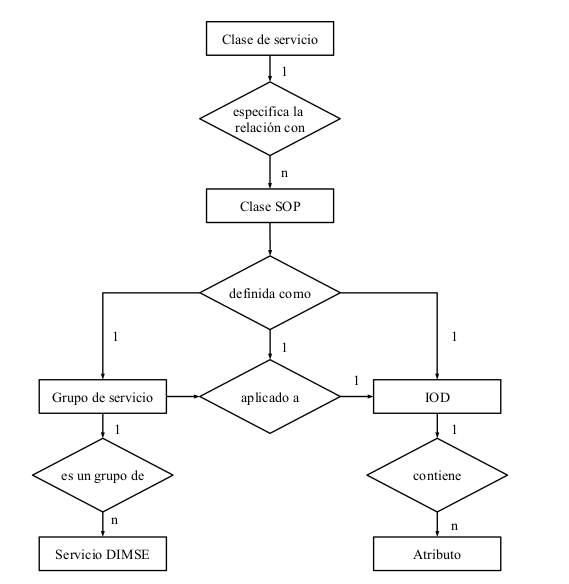
\includegraphics[width=1\textwidth]{images/modeloER_DICOM.png}
\caption{Modelo ER DICOM: Especificación de una clase de servicio}
\label{fig:modeloER_DICOM}
\end{center}
\end{figure}

Cada uno de los grupos de comandos de servicio en DICOM se denominan DIMSE (DICOM Message Service Element). Las \acs{AE}s utilizan estos comandos \acs{DIMSE} para solicitar o proporcionar información de servicio mediante mensajes DICOM. Para ello el estándar define el protocolo \acs{DIMSE}, que establece las reglas de codificación y los procedimientos necesarios para construir estos mensajes utilizados en el intercambio de servicios entre pares de \acs{AE}. Dependiendo del rol asumido por la \acs{AE}, el mensaje generado en base a un comando \acs{DIMSE} puede ser de tipo request (en el rol \acs{SCU}) o response (en el rol \acs{SCP}). Estos dos tipos corresponden con las abreviaturas RQ y RSP, respectivamente \cite{11} \cite{16}.
Un mensaje DICOM presenta una estructura bastante familiar a la de un elemento de datos. La estructura del mensaje se compone de un conjunto de comandos, seguido de un conjunto de datos condicional. El conjunto de comandos es utilizado para indicar las operaciones y/o notificaciones a realizar con o en el conjunto de datos. De forma similar al conjunto de datos en los IODs, un conjunto de comandos se compone de elementos de comando. Cada elemento de comando presenta un campo “tag” explícito, un campo "longitud del valor" y un campo "valor". El conjunto de datos sigue exactamente la misma codificación que se presentó en el subapartado 3.2.2.4 . La figura (Fig. \ref{fig:estructura_msg_DICOM})
muestra la estructura de un mensaje DICOM.

\begin{figure}[!h]
\begin{center}
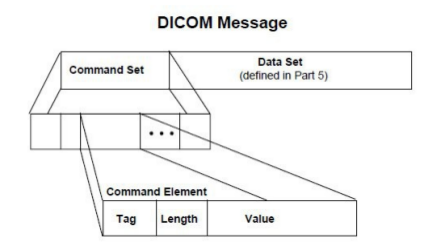
\includegraphics[width=1\textwidth]{images/estructura_msg_DICOM.png}
\caption{Estructura de un mensaje DICOM. Figura extraída de \cite{16}.}
\label{fig:estructura_msg_DICOM}
\end{center}
\end{figure}

A continuación se presentan los servicios \acs{DIMSE} recogidos en el estándar. El contenido de los mensajes, determinado por el protocolo \acs{DIMSE}, varía según la finalidad del comando \acs{DIMSE} en el que esté basado y si se trata de un mensaje RQ o RSP. Para conocer más detalles, esta información puede consultarse en la parte 7 del estándar DICOM (PS3.7) \cite{16}.

Los comandos \acs{DIMSE} especifican \textbf{dos conjuntos de servicios}, según el tipo de información con la que vayan a tratar \cite{11} \cite{16}:

\begin{itemize}
\item \textbf{\underline{Normalizados ( DIMSE-N ):}} Servicios aplicables sólo a IODs normalizados. Estos servicios se concibieron para su uso con registros que representan las propiedades de una sola entidad del mundo real. Presenta las operaciones:
\begin{itemize}
	\item \textbf{N-CREATE (creación)}
	\item \textbf{N-DELETE (borrado)}
	\item \textbf{N-SET (actualización)}
	\item \textbf{N-GET (recuperación)}
	\item \textbf{N-ACTION (operación de un dominio específico que puede ser definida)}
	\item \textbf{N-EVENT\_NOTIFY (servicio de notificación)}
\end{itemize}
\end{itemize}

\begin{itemize}
\item \textbf{\underline{Compuestos ( DIMSE-C ):}} Servicios aplicables sólo a IODs compuestos. Se utilizan en la gestión de documentos que contienen información derivada de más de una entidad del mundo real. Son útiles para la interpretación del intercambio de datos, pues el registro de imágenes es inalterable. Presenta las operaciones:
\begin{itemize}
	\item \textbf{C-FIND \footnote{C-FIND puede ser aplicable tanto a instancias normalizadas como a compuestas.} (consulta)}
	\item \textbf{C-GET (recuperación)}
	\item \textbf{C-MOVE (transferencia)}
	\item \textbf{C-ECHO \footnote{C-ECHO envía una señal a otra AE utilizando el protocolo DICOM para determinar si está conectada conforme a DICOM}(DICOM ping).}
\end{itemize}
\end{itemize}

Una vez se han definido los servicios \acs{DIMSE} y los mensajes \acs{DICOM}, cabe destacar algunas de las clases SOP que se utilizan con mayor frecuencia \cite{10}:
\begin{itemize}
\item \textbf{\underline{Verification SOP:}} Comprueba y valida la conectividad DICOM entre dos AEs.
\end{itemize}

\begin{figure}[!h]
\begin{center}
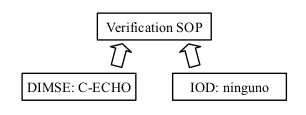
\includegraphics[width=0.5\textwidth]{images/verificacionSOP.png}
\caption{Verificación SOP}
\label{fig:verificationSOP}
\end{center}
\end{figure}

\begin{table}[hp]
\centering{
\small
\begin{tabular}{|l|l|}
\hline
\textbf{Nombre de la clase SOP}	& \textbf{SOP Class UID} \\ \hline
Verification 			& 1.2.840.10008.1.1	 \\ \hline
\end{tabular}
% Local variables:
%   coding: utf-8
%   ispell-local-dictionary: "castellano8"
%   TeX-master: "main.tex"
% End:
}
\caption{Verificación SOP}
\label{tab:verificationSOP}
\end{table}

\begin{itemize}
\item \textbf{\underline{Storage SOP:}} Es el principal responsable de la transferencia de imágenes médicas y otros tipos de datos, entre AEs. DICOM asigna una clase Storage SOP separada a cada modalidad o tipo de dato con su propio UID.
\end{itemize}

\begin{figure}[!h]
\begin{center}
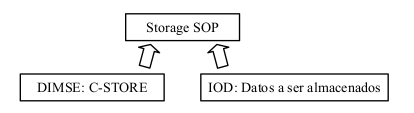
\includegraphics[width=0.5\textwidth]{images/storageSOP.png}
\caption{Storage SOP}
\label{fig:storageSOP}
\end{center}
\end{figure}

En la siguiente tabla (Tabla \ref{tab:storageSOP}) se muestran algunos de los Storage SOPs más utilizados:

\begin{table}[hp]
\centering{
\small
\begin{tabular}{|l|l|}
\hline
\textbf{Nombre de la clase SOP}                            & \textbf{SOP Class UID}      \\ \hline
CR Image Storage                                           & 1.2.840.10008.5.1.4.1.1.1   \\ \hline
Digital X-Ray Image Storage – For Presentation             & 1.2.840.10008.5.1.4.1.1.1.1 \\ \hline
Digital Mammography X-Ray Image Storage – For Presentation & 1.2.840.10008.5.1.4.1.1.1.2 \\ \hline
CT Image Storage                                           & 1.2.840.10008.5.1.4.1.1.2   \\ \hline
\end{tabular}
% Local variables:
%   coding: utf-8
%   ispell-local-dictionary: "castellano8"
%   TeX-master: "main.tex"
% End:
}
\caption{Storage SOP}
\label{tab:storageSOP}
\end{table}

\begin{itemize}
\item \textbf{\underline{Query SOP:}} Dado que la búsqueda de datos de imágenes no es específico de la modalidad de adquisición, DICOM determina \textbf{tres niveles de datos} para la búsqueda de información denominados roots: \textbf{Patient, Study y Patient-Study}. Cada root comienza su búsqueda a partir un nivel en la jerarquía básica de DICOM, por ejemplo, en Patient la búsqueda comenzaría desde Patient-Study-Series-Image y en \textbf{Study (el root por defecto)} sus niveles serían Study-Series-Image, el último root fue retirado del estándar. C-Find presenta un SOP separado para implementar las búsquedas de datos en cada uno de los roots, identificado por su UID.
\end{itemize}

\begin{figure}[!h]
\begin{center}
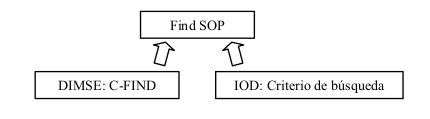
\includegraphics[width=0.5\textwidth]{images/querySOP.png}
\caption{Query SOP}
\label{fig:querySOP}
\end{center}
\end{figure}

\begin{table}[hp]
\centering{
\small
\begin{tabular}{|l|l|}
\hline
\textbf{Nombre de la clase SOP}        & \textbf{SOP Class UID}      \\ \hline
Patient Root Q/R Find                  & 1.2.840.10008.5.1.4.1.2.1.1 \\ \hline
Study Root Q/R Find                    & 1.2.840.10008.5.1.4.1.2.2.1 \\ \hline
Patient-Study Root Q/R Find (Retirado) & 1.2.840.10008.5.1.4.1.2.3.1 \\ \hline
\end{tabular}
% Local variables:
%   coding: utf-8
%   ispell-local-dictionary: "castellano8"
%   TeX-master: "main.tex"
% End:
}
\caption{Query (C-FIND) SOP}
\label{tab:querySOP}
\end{table}

\begin{itemize}
\item \textbf{\underline{Modality Worklist SOP:}} Realiza una precarga de los pacientes y los datos de programación en las modalidades de adquisición.
\end{itemize}

\begin{figure}[!h]
\begin{center}
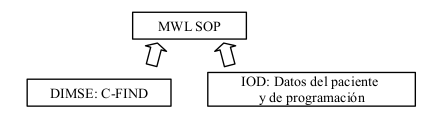
\includegraphics[width=0.5\textwidth]{images/MWSOP.png}
\caption{Modality Worklist SOP}
\label{fig:MWSOP}
\end{center}
\end{figure}

\begin{table}[hp]
\centering{
\small
\begin{tabular}{|l|l|}
\hline
\textbf{Nombre de la clase SOP} & \textbf{SOP Class UID} \\ \hline
Modality Worklist               & 1.2.840.10008.5.1.4.31 \\ \hline
\end{tabular}
% Local variables:
%   coding: utf-8
%   ispell-local-dictionary: "castellano8"
%   TeX-master: "main.tex"
% End:
}
\caption{MWL SOP}
\label{tab:MWSOP}
\end{table}

\begin{itemize}
\item \textbf{\underline{C-Get SOP:}} Recupera las imágenes obtenidas a partir de los atributos de búsqueda especificados, bajo el mismo root definido en el Query SOP. Constituye el \textbf{modo de recuperación básico en \acs{DICOM}}.
\end{itemize}

\begin{figure}[!h]
\begin{center}
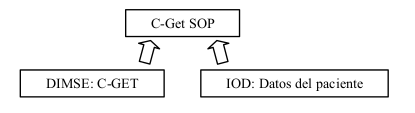
\includegraphics[width=0.5\textwidth]{images/cgetSOP.png}
\caption{C-Get SOP}
\label{fig:cgetSOP}
\end{center}
\end{figure}

C-Get SOP combina \textbf{Query (C-Find) SOP y C-Store SOP} en una única clase de servicio donde las imágenes requeridas pueden ser identificadas sobre la consulta de un C-Find, seguida de una recuperación C-Store. Una clase de servicio que combina estas clases SOP es la clase \textbf{Query/Retrieve} \cite{15}. 

C-Get hereda tres niveles de recuperación (roots) de C-Find que son los recogidos en la siguiente tabla (Tabla \ref{tab:cgetSOP}):

\begin{table}[hp]
\centering{
\small
\begin{tabular}{|l|l|}
\hline
\textbf{Nombre de la clase SOP}       & \textbf{SOP Class UID}      \\ \hline
Patient Root Q/R Get                  & 1.2.840.10008.5.1.4.1.2.1.3 \\ \hline
Study Root Q/R Get                    & 1.2.840.10008.5.1.4.1.2.2.3 \\ \hline
Patient-Study Root Q/R Get (retirado) & 1.2.840.10008.5.1.4.1.2.3.3 \\ \hline
\end{tabular}
% Local variables:
%   coding: utf-8
%   ispell-local-dictionary: "castellano8"
%   TeX-master: "main.tex"
% End:
}
\caption{C-Get SOP}
\label{tab:cgetSOP}
\end{table}

\begin{itemize}
\item \textbf{\underline{C-Move SOP:}} Este SOP es idéntico a C-Get SOP, salvo que en este caso pueden participar otras AEs. Por tanto, recupera las imágenes obtenidas a partir de los atributos de búsqueda especificados, bajo el mismo root definido en el Query SOP, pero los resultados pueden transferirse al mismo AE que inició el C-Move o a otro AE diferente. Constituye el \textbf{modo de recuperación avanzado en \acs{DICOM}}.
\end{itemize}

\begin{figure}[!h]
\begin{center}
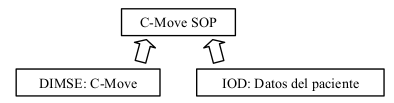
\includegraphics[width=0.5\textwidth]{images/cmoveSOP.png}
\caption{C-Move SOP}
\label{fig:cmoveSOP}
\end{center}
\end{figure}

Al igual que C-Get SOP, C-Move SOP también combina \textbf{Query (C-Find) SOP y C-Store SOP} en una única clase de servicio. La clase de servicio \textbf{Query/Retrieve} también utiliza estas clases \cite{15}.

C-Move también hereda los tres niveles (roots) para la transferencia de imágenes de C-Find:

\begin{table}[hp]
\centering{
\small
\begin{tabular}{|l|l|}
\hline
\textbf{Nombre de la clase SOP}        & \textbf{SOP Class UID}      \\ \hline
Patient Root Q/R Move                  & 1.2.840.10008.5.1.4.1.2.1.2 \\ \hline
Study Root Q/R Move                    & 1.2.840.10008.5.1.4.1.2.2.2 \\ \hline
Patient-Study Root Q/R Move (retirado) & 1.2.840.10008.5.1.4.1.2.3.2 \\ \hline
\end{tabular}
% Local variables:
%   coding: utf-8
%   ispell-local-dictionary: "castellano8"
%   TeX-master: "main.tex"
% End:
}
\caption{C-Move SOP}
\label{tab:cmoveSOP}
\end{table}

La complejidad añadida a C-Move, acerca de la participación de tres AEs en el proceso de búsqueda y recuperación de imágenes, normalmente se utiliza en entornos muy bien controlados. Por ejemplo, cuando desde una estación de trabajo (AE 1) se ordena al sistema de almacenamiento de imágenes (AE 2) que encuentre un estudio de un paciente y lo envíe a otra estación de trabajo o a un servidor específico (AE 3) para su almacenamiento.

\subsubsection{Protocolo \acs{DICOM} Upper Layer}

Bajo el modelo TCP/IP, \acs{DICOM} define un \textbf{mecanismo de asociación} que asegura la comunicación entre dos AEs compatibles y permite transferir los datos en un orden y formato bien definidos. Este mecanismo, también referido como \textbf{protocolo \acs{DICOM UL}}, extiende los servicios proporcionados por el modelo TCP/IP para dirigir las necesidades específicas de \acs{DICOM}.

Toda \textbf{conexión \acs{DICOM}} realizada con éxito presenta \textbf{tres estados:} establecimiento de la asociación, transferencia de datos y finalización de la asociación. El \textbf{servicio A-ASSOCIATE} es usado durante el establecimiento de la asociación. Para la transferencia de datos se utiliza el servicio \textbf{P-DATA.} El estado de finalización de la asociación utiliza uno de los siguientes servicios: \textbf{A-RELEASE y A-ABORT}. Todos estos servicios están soportados por el \textbf{protocolo \acs{DICOM UL}}, el cuál consiste en un conjunto de estructuras específicas para la gestión de la asociación. Estas estructuras se denominan PDU (Protocol Data Unit) \cite{17}.

Al igual que los protocolos del nivel superior, las PDUs siguen el mismo paradigma request-response. En concreto, los comandos de servicio (\acs{DIMSE}) son enviados a la otra AE encapsulados en las PDUs de tipo P-DATA. El estándar presentan las siguientes PDUs para los servicios UL \cite{10}:
\begin{itemize}
\item A-Associate-RQ, petición de asociación \acs{DICOM}
\item A-Associate-AC, aceptación de una petición de asociación \acs{DICOM}
\item A-Associate-RJ, rechazo de una asociación \acs{DICOM}.
\item P-Data-TF, transferencia de un bloque de datos DICOM.
\item A-Release-RQ, petición de asociación terminada.
\item A-Release-RP, respuesta a una petición de asociación terminada.
\item A-Abort, aborta cualquier asociación inválida.
\end{itemize}

El siguiente diagrama (Diag. \ref{fig:comunicacionPDU}) muestra el orden de los estados que suceden en una comunicación \acs{DICOM} entre dos AEs. El inicio de la comunicación se produce al enviar un A-Associate-RQ. Esta PDU contiene una \textbf{"tarjeta de presentación"} de AE1. Si la asociación es aceptada, porque los parámetros enviados por la AE1 están soportados por la AE2, esta última envía un A-Associate-AC con su “tarjeta de presentación”, en caso contrario envía en su lugar un A-Abort y da por concluida la comunicación sin llegar a producirse el segundo estado. En el caso de aceptar la comunicación, se inicia la transferencia de datos entre dispositivos en pequeños trozos P-Data-TF y al final de este estado se procede a cerrar la comunicación con un A-Release-RQ. Los trozos de P-Data-TF encapsulan los comandos de servicio \acs{DIMSE} utilizados para transmitir la información del servicio que se está realizando (codificada mediante atributos de comandos y/o de datos).

Para finalizar este subapartado y a fin de recoger las estructuras utilizadas en el intercambio de información entre AEs, se incluye el siguiente diagrama-ejemplo (Diag. ). Este diagrama corresponde con la \textbf{clase de servicio Query/Retrieve}, en concreto representa el momento en el que se inicia la \textbf{recuperación de imágenes}. En este caso la clase SOP utilizada es \textbf{C-MOVE.} Cuando se inicia la transferencia de imágenes con un C-MOVE-RQ (desde AE1), \textbf{cada imagen es encapsulada en una operación C-STORE separada} y enviada por AE2 a quien solicitó el servicio C-MOVE. También C-MOVE puede enviar a su vez respuestas para informar al SCU del estado de la operación, indicando que se encuentra pendiente de recibir más imágenes. Cuando todas las operaciones C-STORE han sido ejecutadas, C-MOVE responde con un \textbf{C-MOVE-RSP} que indica que \textbf{ha finalizado la recuperación de imágenes.}

\begin{figure}[!h]
\begin{center}
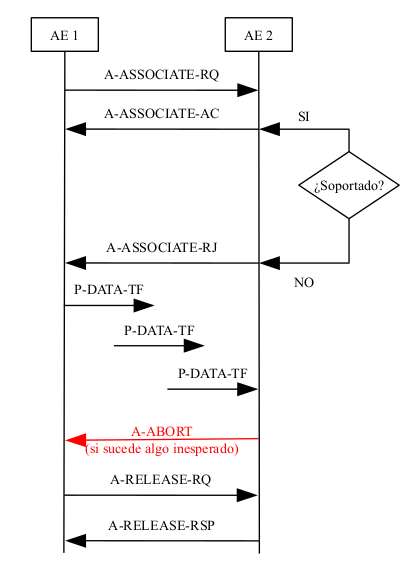
\includegraphics[width=0.85\textwidth]{images/comunicacionPDU.png}
\caption{Comunicación PDU entre dos AEs}
\label{fig:comunicacionPDU}
\end{center}
\end{figure}

% Local Variables:
%  coding: utf-8
%  mode: latex
%  mode: flyspell
%  ispell-local-dictionary: "castellano8"
% End:111111
